\documentclass[12pt]{article}

\usepackage{sbc-template}
\usepackage{graphicx,url}
\usepackage[section]{placeins}
\usepackage{float}
\usepackage[utf8]{inputenc}
\usepackage[brazil]{babel}

\sloppy

\title{Sistema de Locadora de Veículos com ASP.NET Core e Entity Framework}

\author{Samara Lana da Rocha}

\address{Análise e Desenvolvimento de Sistemas -- Pontifícia Universidade Católica de Minas Gerais (PUC Minas)\\
\email{samara.lana@sga.pucminas.br}
}

\begin{document}

\maketitle

\begin{abstract}
This work presents the development of a backend system for a vehicle rental service using ASP.NET Core, Entity Framework, and SQL Server Express. The system allows the management of customers, vehicles, manufacturers, categories, and rentals, providing complete CRUD operations, data validation, and filters with queries involving multiple tables.
\end{abstract}

\begin{resumo}
Este trabalho descreve a implementação de um sistema backend para uma locadora de veículos utilizando ASP.NET Core, Entity Framework e SQL Server Express. O sistema contempla funcionalidades de cadastro, gerenciamento de aluguel e consultas avançadas, garantindo integridade dos dados, organização arquitetural e suporte às principais operações do domínio da locação de veículos.
\end{resumo}

\section{Introdução}

O desenvolvimento de sistemas para locadoras de veículos é importante para automatizar processos operacionais, reduzir erros manuais e melhorar o controle das informações relacionadas ao negócio. Em um cenário de locação, é necessário manter registros confiáveis sobre clientes, veículos, fabricantes, categorias e aluguéis, além de garantir que a disponibilidade dos veículos seja controlada de forma consistente.

Neste contexto, o presente projeto teve como objetivo desenvolver um sistema backend para uma locadora de veículos, utilizando ASP.NET Core, Entity Framework Core e SQL Server Express. A proposta foi construir uma API REST capaz de oferecer operações de cadastro, consulta, atualização e remoção de dados, além de implementar regras de negócio relacionadas ao aluguel e à devolução de veículos.

Entre as principais funcionalidades desenvolvidas, destacam-se o cadastro de clientes, veículos, fabricantes e categorias, o registro de aluguéis e devoluções e a execução de filtros com consultas envolvendo múltiplas tabelas. Como tecnologias principais, foram utilizados C\#/.NET, ASP.NET Core, Entity Framework Core, SQL Server Express e Swagger para testes da API.

\section{Requisitos Funcionais}

O sistema foi projetado para atender às funcionalidades essenciais de uma locadora de veículos. Os requisitos funcionais implementados foram os seguintes:

\begin{itemize}
\item Cadastrar fabricantes de veículos;
\item Cadastrar categorias de veículos;
\item Cadastrar clientes com nome, CPF, e-mail, telefone e data de cadastro;
\item Cadastrar veículos com modelo, ano de fabricação, quilometragem, placa, cor, valor da diária, disponibilidade, fabricante e categoria;
\item Registrar aluguéis associando um cliente a um veículo em um determinado período;
\item Registrar devoluções, informando a quilometragem final e atualizando o valor total da locação;
\item Consultar registros por meio de operações CRUD;
\item Executar filtros envolvendo mais de uma tabela do banco de dados.
\end{itemize}

Os principais casos de uso do sistema são:

\begin{itemize}
\item \textbf{Cadastro de cliente}: permite inserir e consultar clientes da locadora;
\item \textbf{Cadastro de veículo}: permite inserir veículos vinculados a fabricante e categoria;
\item \textbf{Registro de aluguel}: associa cliente e veículo, marcando o veículo como indisponível;
\item \textbf{Registro de devolução}: finaliza o aluguel, calcula o valor total e atualiza a quilometragem do veículo;
\item \textbf{Consulta com filtros}: permite listar veículos por fabricante, veículos por categoria, aluguéis por cliente, aluguéis em aberto e clientes com quantidade de aluguéis.
\end{itemize}

\section{Arquitetura do Sistema}

O sistema foi organizado em uma arquitetura em camadas, com separação de responsabilidades entre os componentes principais da aplicação. Embora não haja interface gráfica, a organização segue uma abordagem semelhante ao padrão MVC, no qual os modelos representam os dados, os controladores concentram a lógica de entrada e saída da API e a camada de persistência realiza a comunicação com o banco de dados.

A estrutura principal do projeto foi dividida da seguinte maneira:

\begin{itemize}
\item \textbf{Models}: contém as classes de entidade do sistema, como Cliente, Veiculo, Fabricante, CategoriaVeiculo e Aluguel;
\item \textbf{Data}: contém a classe \texttt{LocadoraContext}, responsável pela configuração do Entity Framework e do mapeamento com o banco;
\item \textbf{Controllers}: contém os endpoints da API REST, implementando as operações CRUD e os filtros;
\item \textbf{DTOs}: contém classes auxiliares para entrada de dados específicos, como o registro de devolução.
\end{itemize}

Essa divisão favorece a manutenção do sistema, melhora a organização do código e facilita a identificação das responsabilidades de cada parte da aplicação.

\section{Implementação Técnica}

A implementação foi realizada em C\# com ASP.NET Core, utilizando o Entity Framework Core como tecnologia de mapeamento objeto-relacional e o SQL Server Express como banco de dados relacional. Para testes dos endpoints, foi utilizado o Swagger.

As principais tecnologias empregadas foram:

\begin{itemize}
\item C\#/.NET;
\item ASP.NET Core Web API;
\item Entity Framework Core;
\item SQL Server Express;
\item Swagger/OpenAPI.
\end{itemize}

As principais classes do sistema possuem as seguintes responsabilidades:

\begin{itemize}
\item \textbf{Cliente}: representa o cliente da locadora;
\item \textbf{Fabricante}: representa a marca do veículo;
\item \textbf{CategoriaVeiculo}: representa a classificação do veículo;
\item \textbf{Veiculo}: representa os veículos disponíveis para locação;
\item \textbf{Aluguel}: representa a locação de um veículo por um cliente;
\item \textbf{LocadoraContext}: configura o banco de dados, os relacionamentos e as restrições de integridade.
\end{itemize}

Em termos de design, foi adotado o uso de Data Annotations para validação básica de atributos, como obrigatoriedade de campos, tamanho de strings, faixas de valores numéricos e formato de e-mail. Além disso, foram configurados índices únicos para CPF, e-mail, placa e nome da categoria, reforçando a consistência dos dados. Também foi utilizado um enum para representar o status do aluguel, permitindo maior controle semântico sobre os estados possíveis da locação.

\section{Descrição do Banco de Dados}

O sistema foi desenvolvido com persistência em banco de dados relacional utilizando SQL Server Express, sendo o mapeamento objeto-relacional realizado com o Entity Framework Core.

O modelo de dados foi estruturado para atender às necessidades de uma locadora de veículos, contemplando o cadastro de fabricantes, categorias, clientes, veículos e aluguéis. O banco foi projetado com foco em integridade referencial, organização dos relacionamentos e suporte às regras de negócio implementadas na API.

\subsection{Tabelas Principais}

As tabelas principais do sistema são:

\begin{itemize}
\item \textbf{Fabricantes}: armazena as marcas dos veículos cadastrados, contendo informações como nome e país de origem;
\item \textbf{CategoriasVeiculo}: armazena a classificação dos veículos, como SUV, Sedan e Hatch;
\item \textbf{Clientes}: armazena os dados dos clientes da locadora, incluindo nome, CPF, e-mail, telefone e data de cadastro;
\item \textbf{Veiculos}: armazena os dados dos veículos disponíveis para locação, como modelo, ano de fabricação, quilometragem atual, placa, cor, valor da diária e disponibilidade;
\item \textbf{Alugueis}: registra as operações de locação, vinculando cliente e veículo em um determinado período, além de armazenar quilometragem inicial, quilometragem final, valor da diária, valor total e status do aluguel.
\end{itemize}

O banco também possui a tabela técnica \textbf{\_\_EFMigrationsHistory}, criada automaticamente pelo Entity Framework, responsável por armazenar o histórico das migrations aplicadas ao banco.

\subsection{Relacionamentos}

Os relacionamentos entre as entidades foram modelados da seguinte forma:

\begin{itemize}
\item Um \textbf{fabricante} pode estar associado a vários veículos, enquanto cada veículo pertence a apenas um fabricante;
\item Uma \textbf{categoria} pode classificar vários veículos, enquanto cada veículo pertence a apenas uma categoria;
\item Um \textbf{cliente} pode realizar vários aluguéis ao longo do tempo;
\item Um \textbf{veículo} pode participar de vários aluguéis, desde que em períodos diferentes;
\item Cada \textbf{aluguel} está obrigatoriamente associado a um cliente e a um veículo.
\end{itemize}

\subsection{Restrições de Integridade}

Para garantir consistência dos dados, foram adotadas algumas restrições importantes no banco:

\begin{itemize}
\item CPF do cliente com índice único;
\item E-mail do cliente com índice único;
\item Placa do veículo com índice único;
\item Nome da categoria com índice único;
\item Relacionamentos com exclusão restrita, evitando remoção de registros ainda referenciados;
\item Conversão do status do aluguel para texto, facilitando a leitura no banco.
\end{itemize}

Essas restrições foram configuradas no método \texttt{OnModelCreating} da classe \texttt{LocadoraContext}, utilizando recursos do Entity Framework Core.

\subsection{Exemplos de Consultas SQL}

A seguir, são apresentados exemplos de consultas que representam operações importantes no sistema.

Consulta de veículos com seus fabricantes:

\begin{verbatim}
SELECT v.Modelo, v.Placa, f.Nome AS Fabricante
FROM Veiculos v
JOIN Fabricantes f ON v.FabricanteId = f.Id;
\end{verbatim}

Consulta de veículos com suas categorias:

\begin{verbatim}
SELECT v.Modelo, c.Nome AS Categoria
FROM Veiculos v
JOIN CategoriasVeiculo c ON v.CategoriaVeiculoId = c.Id;
\end{verbatim}

Consulta de aluguéis com dados de cliente e veículo:

\begin{verbatim}
SELECT a.Id, cli.Nome AS Cliente, v.Modelo AS Veiculo,
       a.DataInicio, a.DataFimPrevista, a.Status
FROM Alugueis a
JOIN Clientes cli ON a.ClienteId = cli.Id
JOIN Veiculos v ON a.VeiculoId = v.Id;
\end{verbatim}

Consulta de clientes com ou sem aluguel:

\begin{verbatim}
SELECT c.Nome, c.Email, COUNT(a.Id) AS QuantidadeAlugueis
FROM Clientes c
LEFT JOIN Alugueis a ON c.Id = a.ClienteId
GROUP BY c.Nome, c.Email;
\end{verbatim}

\section{Testes e Validação}

Foram realizados testes manuais com os principais endpoints da API utilizando o Swagger. Os testes tiveram como objetivo validar tanto as operações básicas de persistência quanto as regras de negócio implementadas no sistema.

Os testes abrangeram:

\begin{itemize}
\item Inserção de dados por meio de operações POST;
\item Consulta de dados por meio de operações GET;
\item Atualização de dados por meio de operações PUT;
\item Exclusão de registros por meio de operações DELETE;
\item Validação de erros e restrições, como tentativa de cadastro com CPF duplicado;
\item Fluxo de aluguel e devolução de veículos.
\end{itemize}

Durante os testes, foi verificado que a aplicação validava corretamente restrições de unicidade, como no caso de clientes com CPF já cadastrado. Também foram testadas regras específicas de negócio, como o cálculo do valor total do aluguel, a atualização da quilometragem do veículo e a alteração de disponibilidade após a devolução.

Os testes realizados foram predominantemente manuais. Não foram implementados testes automatizados nesta etapa do projeto, de forma que a cobertura concentrou-se na validação funcional dos principais endpoints e fluxos do sistema. Ainda assim, os testes executados foram suficientes para comprovar o funcionamento das operações centrais da aplicação.

\textbf{Inserção de dados (POST)}

\begin{figure}[H]
\centering
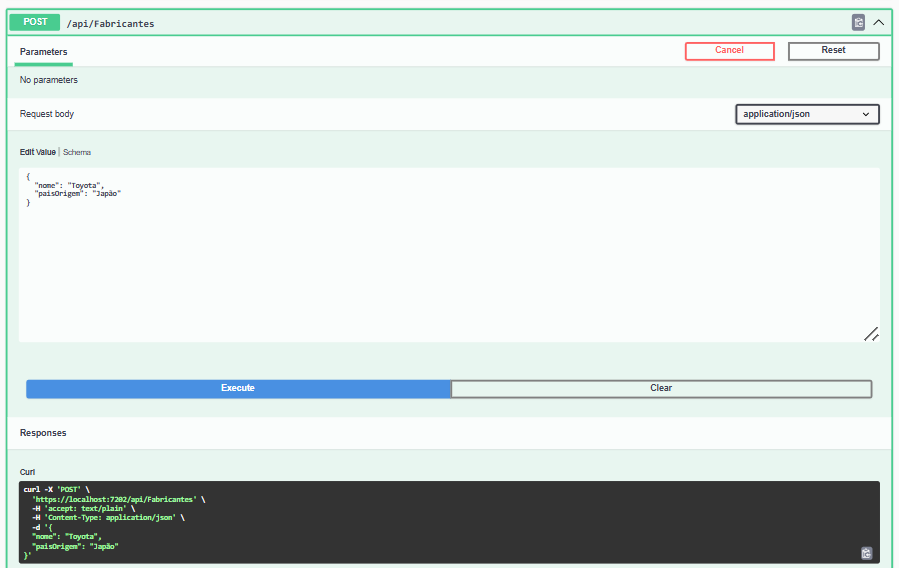
\includegraphics[width=1\linewidth]{fabricantePOST1.png}
\caption{Teste POST Fabricante parte 1}
\end{figure}

\begin{figure}[H]
\centering
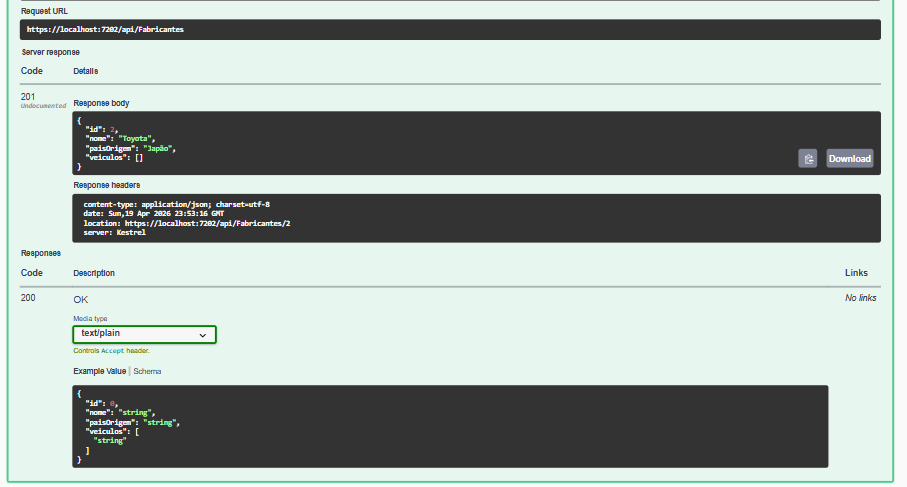
\includegraphics[width=1\linewidth]{image.png}
\caption{Teste POST Fabricante parte 2}
\end{figure}

\begin{figure}[H]
\centering
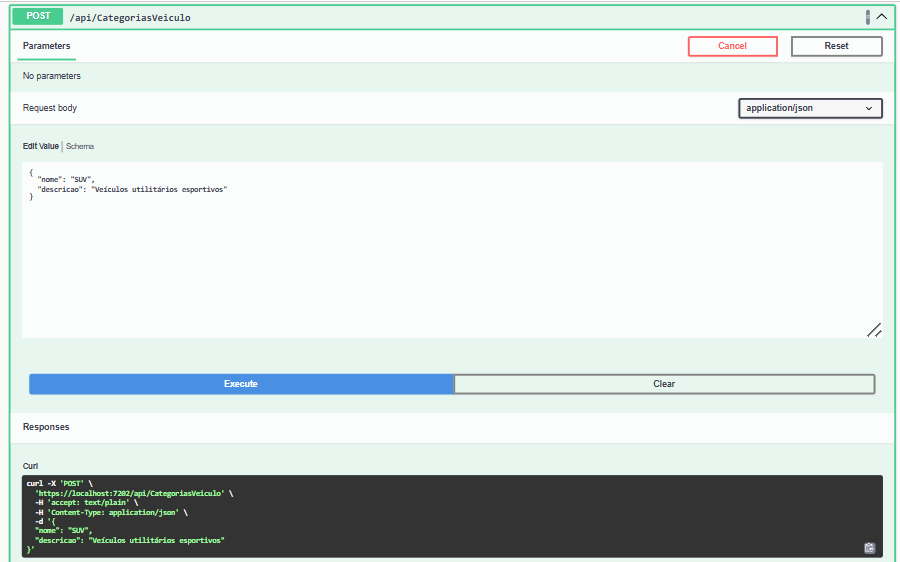
\includegraphics[width=1\linewidth]{categoriaPOST1.png}
\caption{Teste POST Categoria do Veículo parte 1}
\end{figure}

\begin{figure}[H]
\centering
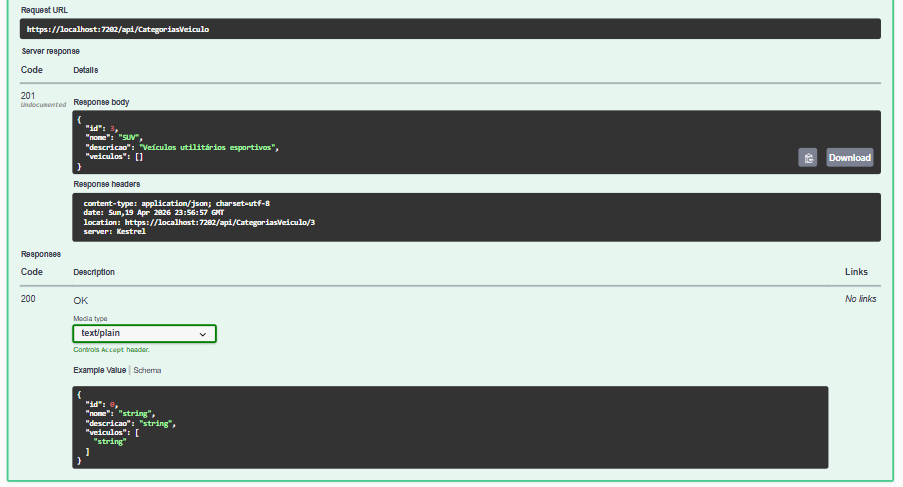
\includegraphics[width=1\linewidth]{categoriaPOST2.png}
\caption{Teste POST Categoria do Veículo parte 2}
\end{figure}

\textbf{Validação de dados (CPF duplicado)}

Durante os testes, foi realizada uma tentativa de cadastro de cliente com CPF já existente, resultando em erro, demonstrando o funcionamento correto da validação.

\begin{figure}[H]
\centering
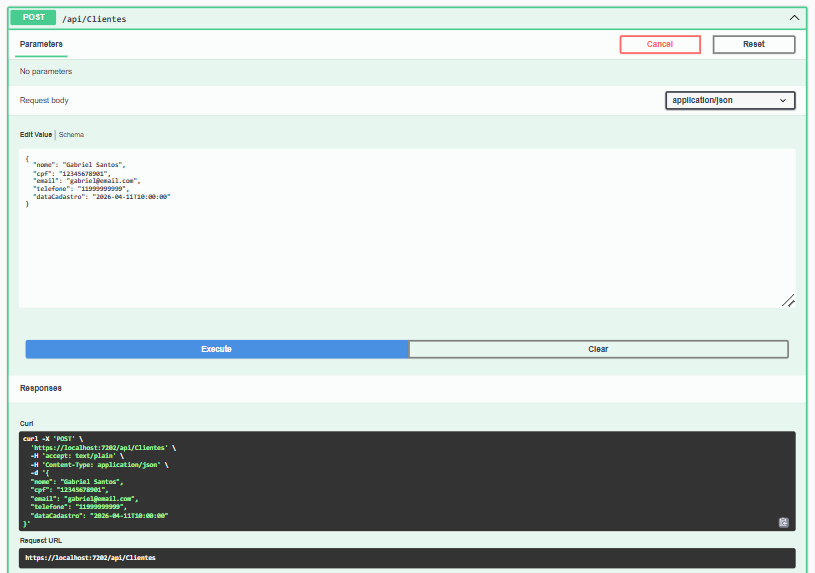
\includegraphics[width=1\linewidth]{tentativaClientePOST1.png}
\caption{Teste POST Cliente com CPF duplicado parte 1}
\end{figure}

\begin{figure}[H]
\centering
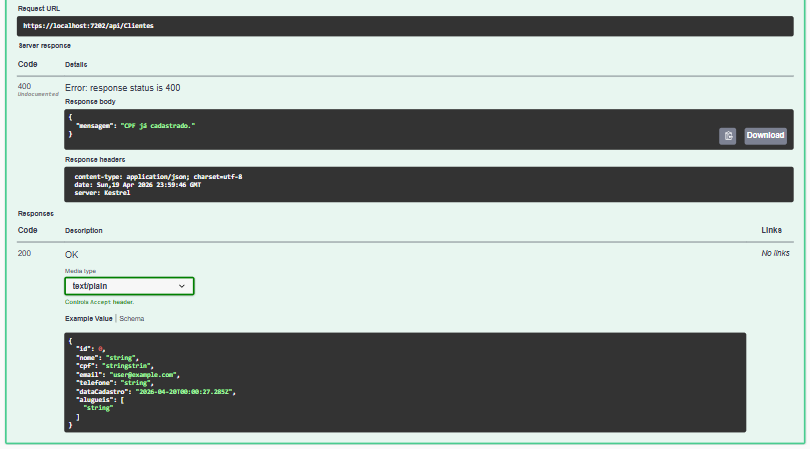
\includegraphics[width=1\linewidth]{tentativaPOSTCliente2.png}
\caption{Teste POST Cliente com CPF duplicado parte 2}
\end{figure}

\textbf{Consultas (GET)}

\begin{figure}[H]
\centering
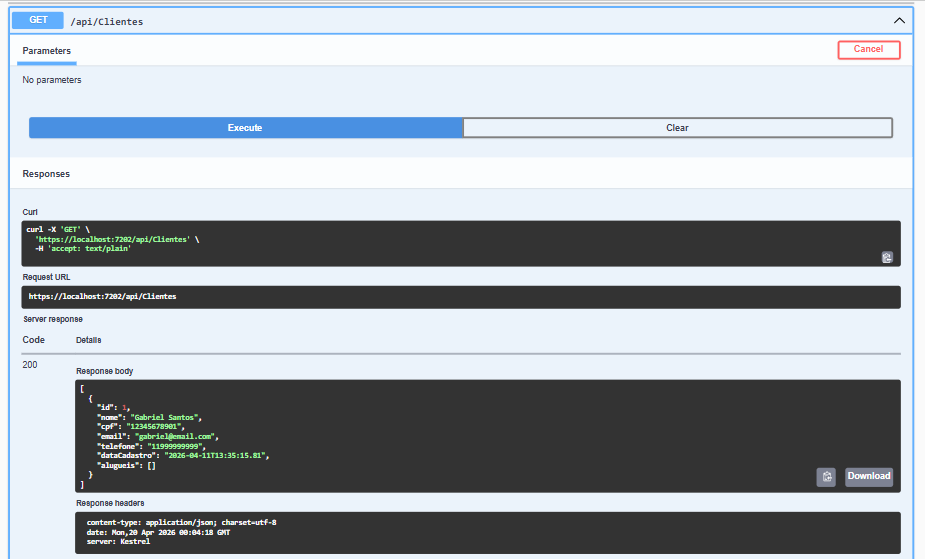
\includegraphics[width=1\linewidth]{clienteGET.png}
\caption{Teste GET Clientes}
\end{figure}

\begin{figure}[H]
\centering
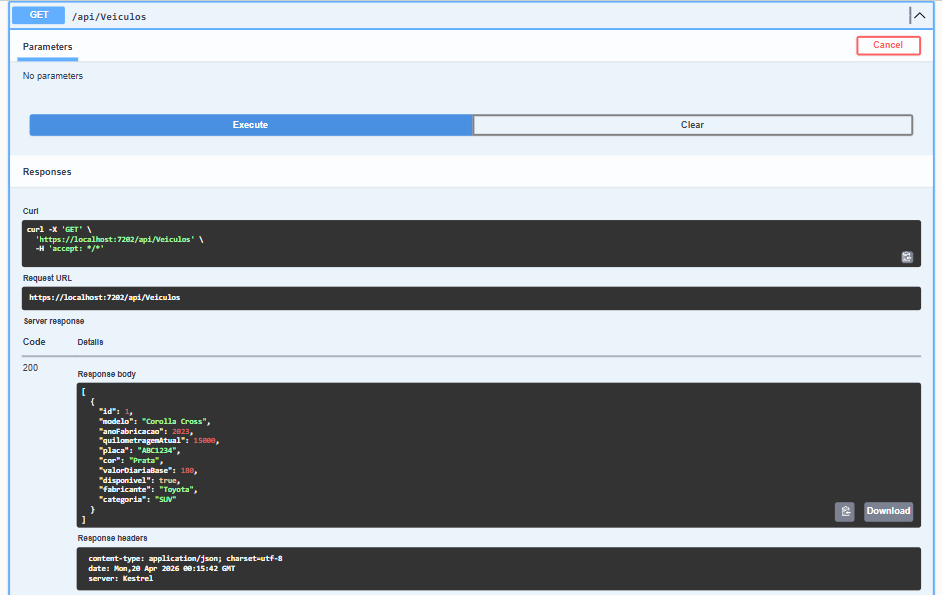
\includegraphics[width=1\linewidth]{veiculoget.png}
\caption{Teste GET Veículo}
\end{figure}

\textbf{Cadastro completo}

\begin{figure}[H]
\centering
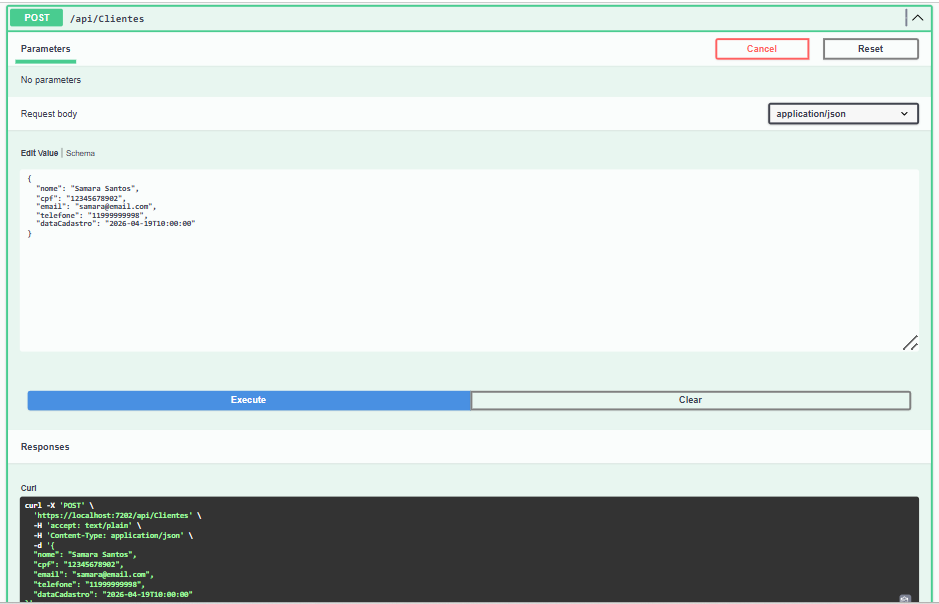
\includegraphics[width=1\linewidth]{clientePOST1.png}
\caption{Teste POST Cliente parte 1}
\end{figure}

\begin{figure}[H]
\centering
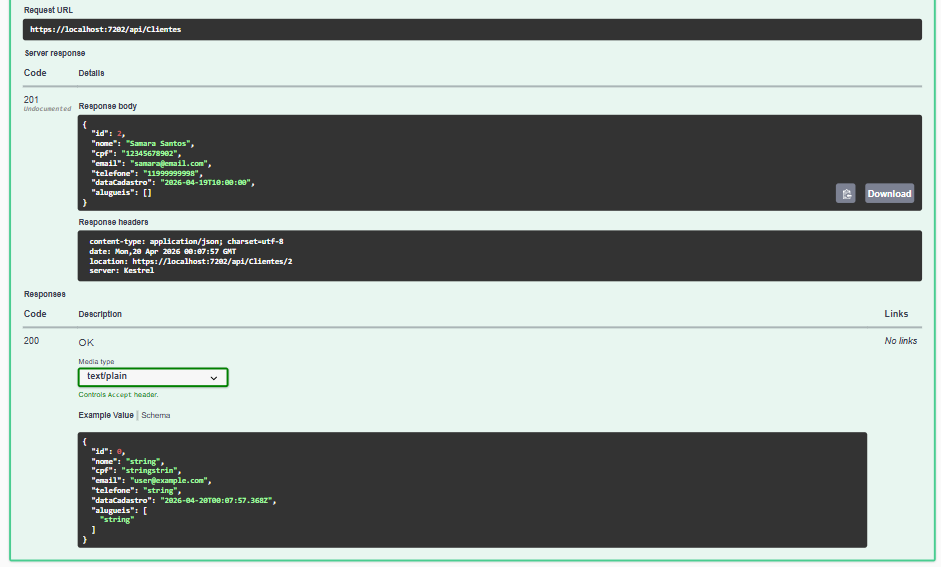
\includegraphics[width=1\linewidth]{clientePOST2.png}
\caption{Teste POST Cliente parte 2}
\end{figure}

\begin{figure}[H]
\centering
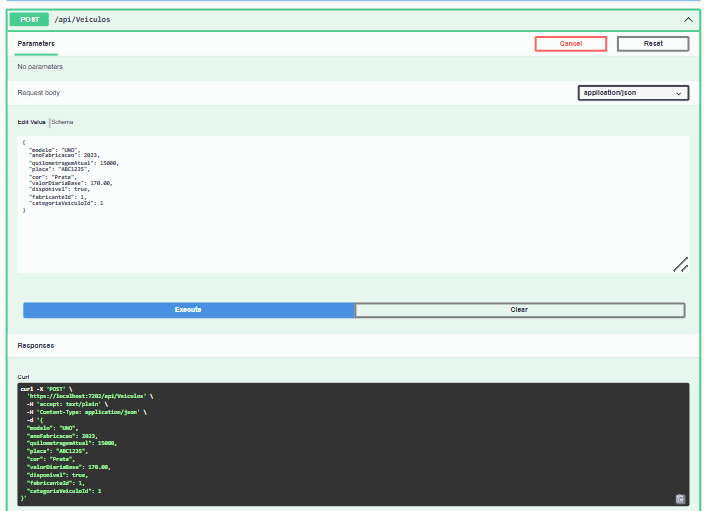
\includegraphics[width=1\linewidth]{veiculoPOST1.png}
\caption{Teste POST Veículo}
\end{figure}

\begin{figure}[H]
\centering
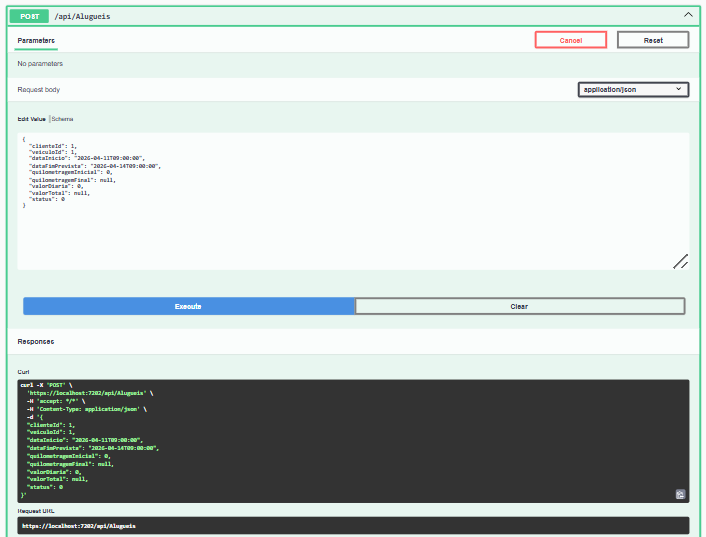
\includegraphics[width=1\linewidth]{aluguelPOST.png}
\caption{Teste POST Aluguel}
\end{figure}

\textbf{Devolução de veículo}

\begin{figure}[H]
\centering
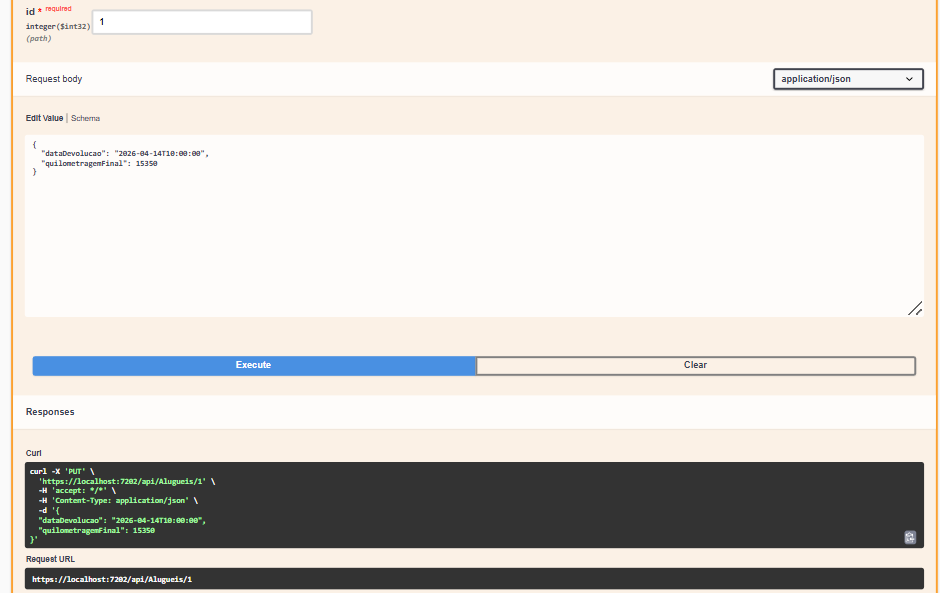
\includegraphics[width=1\linewidth]{devolucao.png}
\caption{Teste PUT Devolução de Aluguel}
\end{figure}

\textbf{Operações adicionais}

\begin{figure}[H]
\centering
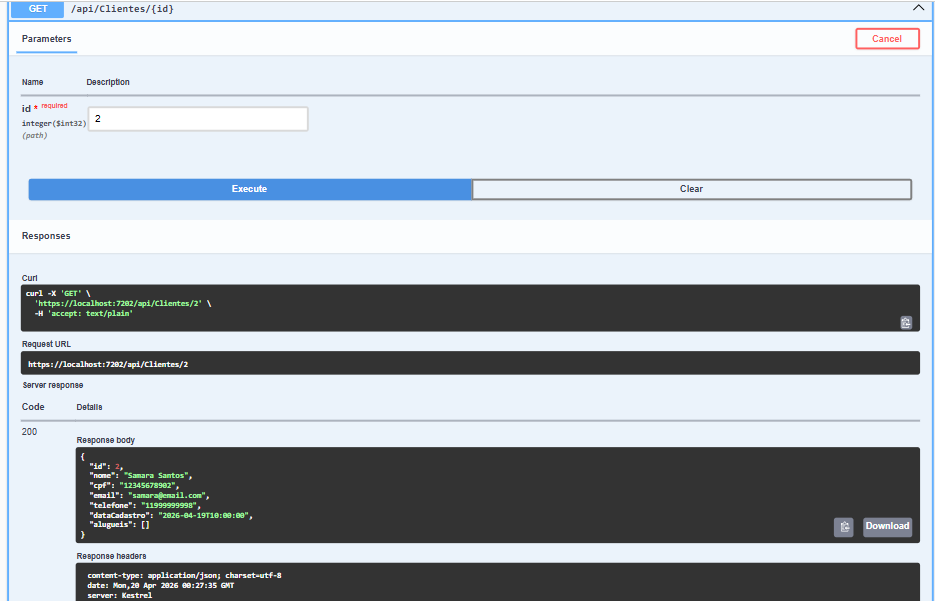
\includegraphics[width=1\linewidth]{getclienteid.png}
\caption{Teste GET Cliente por ID}
\end{figure}

\begin{figure}[H]
\centering
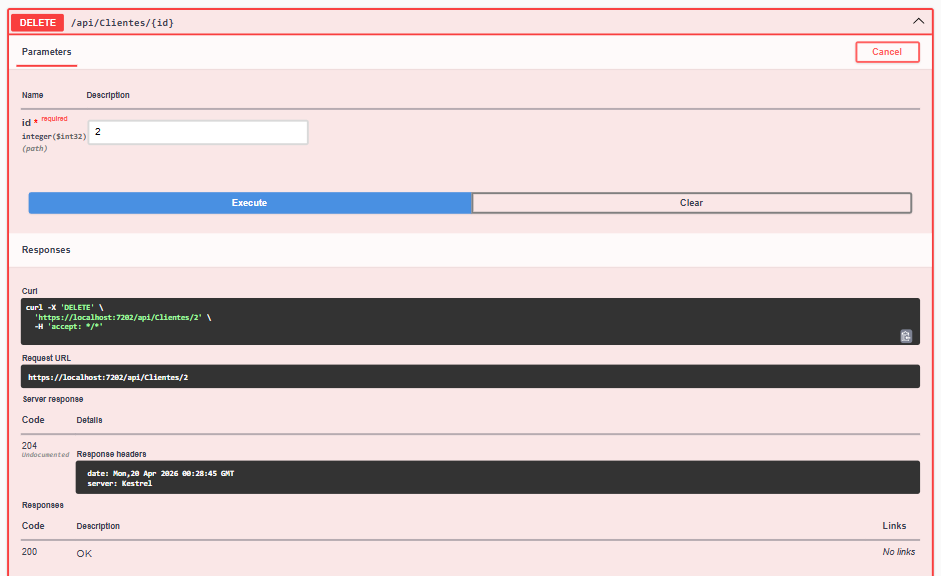
\includegraphics[width=1\linewidth]{CLIENTEDELETE.png}
\caption{Teste DELETE Cliente}
\end{figure}

\FloatBarrier

\section{Resultados e Conclusões}

Os resultados obtidos demonstraram que o sistema atendeu aos requisitos funcionais definidos para o projeto. Foi possível verificar o funcionamento correto dos endpoints de cadastro, consulta, atualização e exclusão, bem como a persistência adequada das informações no banco de dados.

Também foi confirmada a conformidade com requisitos importantes, como o uso do Entity Framework com SQL Server Express, a validação de dados de entrada, a existência de filtros com consultas envolvendo múltiplas tabelas e a implementação das principais regras de negócio do domínio da locadora.

Conclui-se, portanto, que o sistema desenvolvido foi eficaz em atender às necessidades propostas para uma locadora de veículos em nível acadêmico, oferecendo uma base funcional, organizada e coerente com os objetivos do trabalho.

\section{Considerações Finais}

O desenvolvimento deste projeto proporcionou aprendizado prático em modelagem de banco de dados, desenvolvimento de APIs REST, uso do Entity Framework Core, testes com Swagger e organização de um projeto backend em camadas.

Além do ganho técnico, a experiência contribuiu para o entendimento da integração entre banco de dados e aplicação, bem como para a aplicação de conceitos estudados em sala em um contexto prático.

Como melhorias futuras, destacam-se:

\begin{itemize}
\item Desenvolvimento de interface gráfica para interação com o sistema;
\item Implementação de autenticação e controle de acesso;
\item Inclusão de relatórios gerenciais;
\item Expansão da cobertura com testes automatizados.
\end{itemize}

\section{Referências}

\begin{flushleft}

MICROSOFT. \textit{ASP.NET Core Documentation}. Disponível em: 
\url{https://learn.microsoft.com/aspnet/core}. Acesso em: 10 abr. 2026.

MICROSOFT. \textit{Entity Framework Core Documentation}. Disponível em: 
\url{https://learn.microsoft.com/ef/core}. Acesso em: 10 abr. 2026.

MICROSOFT. \textit{SQL Server Documentation}. Disponível em: 
\url{https://learn.microsoft.com/sql}. Acesso em: 10 abr. 2026.

SMARTBEAR. \textit{Swagger Documentation}. Disponível em: 
\url{https://swagger.io/docs}. Acesso em: 10 abr. 2026.

\end{flushleft}

\end{document}